\documentclass{article}
\usepackage[utf8]{inputenc}

\usepackage[utf8]{inputenc}
\usepackage[paperwidth=8.5in, paperheight=11in, top=1in, bottom=.5in, left=.5in, right=.5in]{geometry}
\usepackage{fancyhdr, graphicx,tikz}


\pagestyle{fancy}
\lhead{\large{\textbf{Limits - Readiness Assurance Test}}}
\chead{}
\rhead{}
\lfoot{}
\cfoot{}
%\rfoot{\thepage/\pageref{LastPage} }

\begin{document}




\begin{enumerate}
    \item Suppose that $q = f(p)$, so that the quantity $q$ is a function of the quantity $p$. Let's say the dependent variable has value 10 when the independent variable has value 2. Which equation best expresses this relationship?
    \begin{enumerate}
        \item 2 = f(10)
        \item 10 = f(2) %correct
        \item ...
        \item ...
    \end{enumerate}
    
    \item Simplify the following expression:
        \[  \frac{x^2-6x+8}{x^2-5x+6}
        \]
        \begin{enumerate}
            \item $\displaystyle \frac{(x-4)}{(x-3)}$ %correct
            \item b
            \item c
            \item d
            \item e
        \end{enumerate}
        
    \item Find all vertical asymptote(s), horizontal asymptote(s), and hole(s) for the function given below.
        \[ f(x) = \frac{x^2-6x+8}{x^2-5x+6}
        \]
        
        \begin{enumerate}
            \item vertical asymptote of $x=3$, horizontal asymptote of $y=1$, hole when $x=2$ %correct
            \item vertical asymptote of $x=2$, horizontal asymptote of $y=1$, hole when $x=3$
            \item vertical asymptote of $x=2$, horizontal asymptote of $y=1$, hole when $x=3$
            \item some more mix up
        \end{enumerate}
    
    \item Use interval notation to represent the number line shown below.
    \begin{center}
            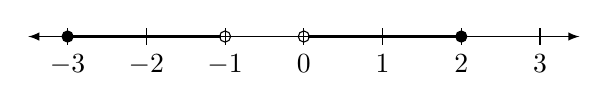
\begin{tikzpicture}
            \draw[latex-latex] (-3.5,0) -- (3.5,0) ; %edit here for the axis
            \foreach \x in  {-3,-2,-1,0,1,2,3} % edit here for the vertical lines
            \draw[shift={(\x,0)},color=black] (0pt,3pt) -- (0pt,-3pt);
            \foreach \x in {-3,-2,-1,0,1,2,3} % edit here for the numbers
            \draw[shift={(\x,0)},color=black] (0pt,0pt) -- (0pt,-3pt) node[below] 
            {$\x$};
            \draw[very thick] (-3,0) -- (-1.05,0);
            \filldraw (-3,0) circle (2pt);
            \draw (-1,0) circle (2pt);
            \draw[very thick] (0.05,0) -- (1.95,0);
            \filldraw (2,0) circle (2pt);
            \draw (0,0) circle (2pt); 
            \end{tikzpicture}
        \end{center}
    
    
        \begin{enumerate}
            \item $[-3,2]$
            \item $[-3,-1) \cup (0,2] $ %correct
            \item $(-3,-1) \cup (0,2) $
            \item $(-3,-1] \cup [0,2) $
            \item $[-3,-1] \cup [0,2] $
        \end{enumerate}
    
    \item
    
    \item Which expression is equal to the product $(x-4)(x^2+3x-3)$?
    \begin{enumerate}
        \item $x^3 - x^2 - 15 x + 12$ % correct
        \item $x^2 + 4x - 7$ %added rather than multiplied
        \item need a bit of time to find good distractors
    \end{enumerate}
    
    \item
    
    \item Consider the function $h(x)$ whose graph is pictured below. Select the most accurate statement.
    
    \includegraphics[keepaspectratio=True, width=0.3\linewidth]{images/eval-dom-rng.png}
    \begin{enumerate}
        \item $h(1) = 3$
        \item $h(2) = 3$ %correct
        \item $h(3) = 2$
        \item $h(4) = 1$
    \end{enumerate}
    
    \item 
    
    \item (10) What is the domain of the function
    \[
        \frac{x-1}{x+1} + \frac{x+3}{x-4}?
    \]
    \begin{enumerate}
        \item All real numbers
        \item All real numbers except $1$ and $-4$
        \item All real numbers except $1$ and $-3$
        \item All real numbers except $-1$ and $4$ %correct
        \item All real numbers except $-1$ and $3$
    \end{enumerate}
    
    
\end{enumerate}


\end{document}
